\section{Introduction}\label{sec:intro}

\subsection{The problem}\label{sec:intro-problem}

Points of $\R^{2n}=\C^n$ are $z=(z_1,\dots,z_n)$, $z_j=x_j+iy_j$, the symplectic form is
$\omega_0=\sum_jdx_j\wedge dy_j$, and the Hamiltonian vector field of a function $H(t,z)$ is defined by
$\iota_{X_H}\omega_0=dH$, i.e.\ $X_H=(\partial_{y_1}H,\dots,\partial_{y_n}H,-\partial_{x_1}H,\dots,
-\partial_{x_n}H)$ in the coordinates $(x,y)$. An integral curve of $X_H$ is a differentiable
$\gamma$ with $\gamma'(t)=X_H(t,\gamma(t))$, and $\phi^t_H$ denotes the flow of $X_H$ from time $0$ to
time $t$. We write $B(c)$ for the closed ball of capacity $c$, that is $\{\pi|z|^2\le c\}$, $\Bo(c)$ for its interior,
and $B(s,c)=s+B(c)$ for $s\in\R^{2n}$.

A \emph{symplectic packing} of a ball by finitely many balls is a family of symplectic embeddings of the balls into
the ball with pairwise disjoint images. Since $\vol B(c)=c^n/n!$, balls of capacities $c_1,\dots,c_k$ can be packed
into $\Bo(C)$ only if $\sum_ic_i^n<C^n$, and Gromov's two-ball theorem \cite{Gromov1985} gives the second obstruction
$c_i+c_j<C$ for $i\ne j$. In dimension four there are further obstructions: five balls of capacity $\frac{11}{25}$
satisfy both inequalities, but the fifth ECH capacity of their union is at least $\frac{11}5$, and that of $\Bo(1)$ is
$2$ \cite{Hutchings2011}.

In dimension four the existence question is settled. Biran \cite{Biran1997} showed that for every $k\ge9$ and every $c$
with $kc^2<C^2$, $k$ balls of capacity $c$ embed in $\Bo(C)$, and the work of McDuff--Polterovich, McDuff, Li--Liu and
Li--Li \cite{McDuffPolterovich1994,McDuff1998,LiLiu2001,LiLi2002} reduces every four-dimensional ball packing problem to
a list of inequalities indexed by exceptional classes. These proofs use $J$-holomorphic curves and, through Taubes'
theorem and inflation on blow-ups of $\CP^2$, Seiberg--Witten theory. They show that embeddings exist; they do not
produce a Hamiltonian that moves given balls into the target. Explicit full packings for square $k$, and several other constructive methods, are discussed in
\S\ref{sec:intro-prior}. Here the goal is one Hamiltonian construction for every $k\ge10$ and every positive error.

Epoch AI \cite{Epoch} asked for such a motion: for every integer $k\ge10$ and every $\eps\in(0,1)$, an algorithm
that, on input $(k,\eps)$, outputs an explicit smooth time-dependent Hamiltonian $H(t,z)$ on $\R^4$ whose time-one map sends the closed unit
balls centred at $(3i-3,0,0,0)$, $1\le i\le k$, into a closed ball $B^4(R)$ of Euclidean radius $R$ centred at the
origin, with $k/R^4>1-\eps$. Since the flow preserves volume, $k/R^4$ is the fraction of $B^4(R)$ filled by the
images. The construction below supplies one Hamiltonian for each $(k,\eps)$, defined by the same formulas
for all of them; Theorem~\ref{thm:eff-algorithm} supplies a uniform algorithm with finite output.
Remark~\ref{rem:eff-epoch-interface} relates these results to Epoch's program submission format.

\subsection{The four-dimensional theorem}\label{sec:intro-contribution}

For admissible data (Definition~\ref{def:intro-admissible}) we define in \S\ref{sec:ham} one Hamiltonian
$H[n,k,C,c,s]$ (Definition~\ref{def:ham-H-final}), by a construction that is the same for all data. The first theorem is its
four-dimensional instance for the data of the Epoch question.

\begin{maintheorem}[Equal balls in the four-ball]\label{thm:intro-4d}
\uses{def:ham-H-final, def:intro-spec, prop:cmp-linear, thm:main}
Let $k\ge10$ be an integer and $\eps\in(0,1)$. Put
\[
 R=\left(\frac{k}{1-\eps/4}\right)^{1/4},\qquad C=\pi R^2,\qquad s_i=(3i-3,0,0,0)\in\R^4\quad(1\le i\le k),
\]
and $H_{k,\eps}=H[2,k,C,(\pi,\dots,\pi),(s_1,\dots,s_k)]$. Then $H_{k,\eps}$ is $C^\infty$ on $\R\times\R^4$, vanishes
for $t\notin(0,1)$ and outside $\R\times\mathcal S$ for an explicit compact set $\mathcal S$, and satisfies
$\Pack(2,k,C,(\pi,\dots,\pi),s)$ (Definition~\ref{def:intro-spec}): its flow is global, and its time-one map sends each
closed unit ball $B(s_i,\pi)$ into $\Bo(\pi R^2)$, the open Euclidean ball of radius $R$ about the origin, with pairwise
disjoint images. Moreover $k/R^4=1-\eps/4>1-\eps$.
\leanmark{four\_dim\_theorem, main\_time\_support, main\_support\_radius, flow\_images\_disjoint}
\end{maintheorem}

\begin{proof}
The centres are at distance at least $3$, so the closed unit balls are disjoint. Since $R^4=k/(1-\eps/4)>k\ge10$, we
have $k\pi^2<\pi^2R^4=C^2$ and $3\pi<\pi R^2=C$, so $(2,k,C,(\pi,\dots,\pi))$ is admissible and
Theorem~\ref{thm:main}(i) below applies. For these data the normalised capacity $\rho=\pi/C=R^{-2}$ satisfies
$\rho\sqrt k=\sqrt{1-\eps/4}>\sqrt3/2>\frac34$, which selects the linear comparison datum of
Proposition~\ref{prop:cmp-linear} in \Sref{Construction}{cons:ham-branch}.
\end{proof}

The theorem leaves an explicit margin. The images lie in the closed ball of radius $R$, while the density requirement
$k/R'^4>1-\eps$ is already met by $R'=(k/(1-\eps/2))^{1/4}>R$. The following estimate converts this margin, a closed
formula in $(k,\eps)$, into a tolerance on the vector field.

\begin{mainproposition}[Robustness]\label{thm:intro-stability}
Let $k\ge10$, $\eps\in(0,1)$, and let $R<R'$ be as above. Let $\widehat H$ be a smooth function on $\R\times\R^4$
vanishing outside $\R\times K$ for a compact set $K$. Suppose that, for $t\in[0,1]$, the field $X_{\widehat H}(t,\cdot)$
is $L$-Lipschitz for some $L\ge0$ and $|X_{\widehat H}-X_{H_{k,\eps}}|\le\eta$ on $\R^4$, where $\eta e^L\le R'-R$. Then the time-one map
of $\widehat H$ sends each closed unit ball $B(s_i,\pi)$ into the closed ball of radius $R'$ about the origin, and
$k/R'^4=1-\eps/2>1-\eps$.
\leanmark{four\_dim\_stability}
\end{mainproposition}

\begin{proof}
Let $\gamma$ and $\hat\gamma$ be integral curves of $X_{H_{k,\eps}}$ and $X_{\widehat H}$ starting at the same point of
$B(s_i,\pi)$. Then $|\hat\gamma(1)-\gamma(1)|\le\eta(e^L-1)/L\le\eta e^L$ by Gr\"onwall's inequality
(Lemma~\ref{lem:eff-gronwall}, with the Lipschitz bound on $X_{\widehat H}$), and $|\gamma(1)|\le R$ by
Theorem~\ref{thm:intro-4d}. For $L=0$ the Gr\"onwall bound is $\eta$.
\end{proof}

Thus every smooth compactly supported approximation with vector-field error at most $(R'-R)e^{-L}$ still meets the
Epoch requirement, with images in the ball of radius $R'$; the geometric margin $R'-R$ depends only on $(k,\eps)$. Theorem~\ref{thm:eff-algorithm} gives one
algorithm which, on input $k$ and a name of $\eps$, halts with $B\in\N$ and $P\in\Q[t,z]$ such that $\beta_B\cdot P$, a
rational polynomial times a fixed smooth cutoff, satisfies the same packing specification. Each output is certified by
a finite rational test, and the construction shows that the search terminates.

The packings of Theorem~\ref{thm:intro-4d} exist by Biran's theorem. The proof here works with explicit maps, forms and
flows only and uses none of the existence results quoted above. Through Corollary~\ref{thm:main-equal} it gives a proof
of Biran's packing stability for $B^4$ without $J$-holomorphic curves or Seiberg--Witten theory, which the earlier
proofs \cite{Biran1997,Biran1999,BuseHind2013,BuseHindOpshtein2016} use, directly or through the results they cite.

\subsection{The mechanism}\label{sec:intro-mechanism}

The construction follows a mechanism due to the OpenAI preprint \cite{OpenAI2026}. We describe it in dimension four, where the picture is
classical. Give $\CP^2$ the Fubini--Study form for which a line has area $1$, so that $\vol\CP^2=\frac12$ and the
complement of a line is $\Bo(1)$. Let $E\subset\CP^2$ be a smooth cubic, of area $3$. Biran \cite{Biran2001} showed
that the complement of an isotropic skeleton in $\CP^2$ is symplectomorphic to a disc bundle over $E$: the normal
bundle, of degree $E\cdot E=9$, with fibre discs of capacity $\frac13$. With fibre moment $p=\pi|w|^2$, the base area
of the circle bundle at level $p$ is
\[
 A(p)=3-9p=3(1-3p)\qquad(0\le p<\tfrac13),\qquad \int_0^{1/3}A(p)\,dp=\frac12=\vol\CP^2 .
\]
The cubic is the first smooth plane curve with the topology needed by this handle construction. Its closed base
must carry a closed one-form $\beta$ with nonzero period around the handle. A line or conic has genus zero, so
$H^1(S^2;\R)=0$ rules out such a form; a cubic has genus one. Thus the fibre bound $\frac13$, and hence $3c_i<C$,
reflects the choice of the smallest-degree smooth plane curve supporting this mechanism.

A ball $B(a)\subset\C\times\C$, sliced by the moment $p$ of its second coordinate, is a family of discs of capacity
$a-p$ for $p\le a$; its slice profile is $(a-p)_+$, and $\int_0^\infty(a-p)_+\,dp=a^2/2=\vol B(a)$. Placing balls
fibrewise in the bundle requires $a<\frac13$: this is the source of the condition $3c_i<C$. If
$\sum_i(a_i-p)_+\le A(p)$ for every $p$, the base discs can be placed side by side over $E$. For nine balls of
capacity $\frac13$ this holds with equality. For $k\ge10$ balls of capacity close to $1/\sqrt k$ the integrated
inequality $\sum_ia_i^2/2<\frac12$ holds, but at $p=0$ one needs $\sum_ia_i\le3$, which fails: the difference
$A(p)-\sum_i(a_i-p)_+$ has positive integral and is negative near $p=0$ (Figure~\ref{fig:intro-profile}).

\begin{figure}[ht]
\centering
\begin{tikzpicture}[x=27cm,y=1.15cm,font=\footnotesize]
 % deficit and surplus regions for k=13, a=0.99/sqrt(13)=0.2746, h=0.33
 \fill[black!25] (0,3) -- (0,3.570) -- (0.1424,1.718) -- cycle;
 \fill[black!8] (0.1424,1.718) -- (0.2746,0) -- (0.33,0) -- (0.33,0.03) -- cycle;
 \draw[->] (0,0) -- (0.36,0) node[right] {$p$};
 \draw[->] (0,0) -- (0,3.9);
 \draw[thick] (0,3) -- (0.3333,0);
 \draw[thick,dashed] (0,3.570) -- (0.2746,0);
 \draw (0.3333,0) -- (0.3333,-0.08) node[below] {$\tfrac13$};
 \draw (0.2746,0) -- (0.2746,-0.08) node[below] {$a$};
 \draw (0,3) -- (-0.004,3) node[left] {$3$};
 \node[right] at (0.06,3.4) {$\sum_i(a_i-p)_+$};
 \node[right] at (0.2,1.45) {$A(p)=3-9p$};
 \node at (0.035,2.95) {$-$};
 \node at (0.27,0.25) {$+$};
\end{tikzpicture}
\caption{The area profile $A$ of the cubic model (solid) and the slice profile of $13$ balls of capacity
$a=0.99/\sqrt{13}$ (dashed). The deficit (dark) is smaller than the surplus (light), since
$\int_0^h(A-\sum_i(a_i-p)_+)\,dp=\frac12(1-13a^2-(1-3h)^2)>0$ for $h=0.33$, but stacking needs $A\ge\sum_i(a_i-p)_+$
pointwise. The twist moves area from the surplus to the deficit.}
\label{fig:intro-profile}
\end{figure}

The construction of \cite{OpenAI2026} pays the deficit with the surplus by twisting the bundle. Across an
annulus in the base, the fibre over one boundary circle is identified with the fibre over the other by an
area-preserving map $q$ of the fibre disc instead of the identity. Paired with a function $K$ of the moment, the
twist changes the base area available above a fibre point $w$ from $A(p(w))$ to
$A(p(w))+K(p(q^{-1}w))-K(p(w))$ (equation~\eqref{eq:mech-available}). Since $q$ preserves the fibre area, this
redistributes area between moment levels without changing the total. The balls fit if, for some $\gamma>0$ and
$P=A-\sum_i(a_i-p)_+$,
\[
 (K-P)\bigl(p(q(w))\bigr)\le K\bigl(p(w)\bigr)-\gamma\qquad\text{for every fibre point }w.
\]
This forces $\int P>0$. Conversely, for concave $P$ with positive mean that is positive outside a core,
\cite{OpenAI2026} obtains $K$ as the fixed point of a contraction built from increasing rearrangements, realises the
rearrangements by isotopies, and turns the inequality into embeddings by Moser's method and a transfer to the target.
For $k\ge10$ equal balls with $\frac34<\rho\sqrt k<1$ a linear $K$ suffices: $K-P$ is, up
to a constant, a tent whose increasing rearrangement is linear, and the inequality becomes an identity up to the error
of one planar map (Proposition~\ref{prop:cmp-linear}).

\subsection{The main steps}\label{sec:intro-steps}

The four-dimensional contribution consists of four constructions, listed in Table~\ref{tab:intro-steps}: the linear
comparison identity, which removes the fixed-point step for the Epoch family; an explicit planar rearrangement; a
symmetry-controlled return from the Fermat cubic model, written in explicit cover coordinates, to the affine ball;
and one global motion from the prescribed source balls. We first give the construction chain for
Theorem~\ref{thm:intro-4d}.

\emph{The construction chain.} After the dilation by $1/\sqrt C$ the target is $\Bo(1)$ and each ball has capacity $\rho$.
Put $\eta_\star=1-\sqrt{1-\eps/4}$, $t_0=1-\eta_\star/2$, $a=t_0/\sqrt k$, $h=t_0/3$ and $g=3\eta_\star/2$. Then $H_{k,\eps}$ is
obtained in five steps, each determined by the data and by the previous steps.
\begin{enumerate}[label=(\arabic*)]
\item \emph{Model.} The cubic disc-bundle model associated with Biran's decomposition, written on the cover $\R^2\times\C$ of the Fermat torus with the
 explicit form $\Omega_0$ of \S\ref{sec:mdl-cub}, cut at fibre moment $p\le h$.
\item \emph{Comparison.} The linear function $K(p)=(3\sqrt k-9)p$ and the fibre isotopy $(q_t)$ of
 \Sref{Theorem}{thm:pll-inner}, generated by an explicit planar Hamiltonian; its endpoint carries the centred disc of
 area $I$ into the sublevel set $\{\Lambda\circ p\le I+4e_q\}$ of the tent $\Lambda$ of \S\ref{sec:cmp-linear}, with $e_q$ as there. The
 comparison gap is $\frac{31}{32}g$ (Proposition~\ref{prop:cmp-linear}).
\item \emph{Handle.} Over an annulus $\mathcal A$ in the base, the bundle chart $\chi_{\mathcal A}$ and the twist
 $\mathcal D$, which applies $q_{f(s)}$ to the fibre over the handle coordinate $s$ for a fixed clock $f$; the Moser map
 $\Phi$, the time-one map of three explicit fields; the layer maps $E_i$, given by an explicit strip map and unique
 roots (\S\ref{sec:hdl}, Remark~\ref{rem:hdl-four}).
\item \emph{Return.} The map $\mathcal T=b_{\rm ball}\circ\psi_1^{-1}\circ\mathrm{pr}\circ\tau_1\circ\iota\circ\mathsf N$
 from the model into $\Bo(1)$: it carries the model into $\CP^2$ minus the line $\{Z_0=0\}$, which the ball chart
 $b_{\rm ball}$ identifies with $\Bo(1)$; $\tau_1$ and $\psi_1$ are time-one maps of explicit ordinary differential
 equations (\Ssec{sec:rtc}). The embeddings are
 \[
  f_i(u)=\sqrt C\,\bigl(\mathcal T\circ\Phi^{-1}\circ\chi_{\mathcal A}\circ\mathcal D^{-1}\circ E_i\bigr)(u/\sqrt C)
 \]
 (\Sref{Remark}{rem:cub-lean}).
\item \emph{Motion.} One isotopy $F_{i,t}$ from the translations $u\mapsto s_i+u$ to the $f_i$, with disjoint images at all
 times (Proposition~\ref{prop:ham-isotopy}), and $H_{k,\eps}$, the pushforward along it of a radial primitive computed in
 the source balls (Definition~\ref{def:ham-H}).
\end{enumerate}
The parameters $t_0$, $a$, $h$, $g$, the slope of $K$ and the height $d_n=\frac13-\frac{\eta_\star}{12}$ used by the return are
closed-form expressions in $\sqrt k$ and $\eps$ (\Sref{Remark}{rem:rtc-equal}); the maps are formulas, integrals,
time-one maps of explicit vector fields, inverses of explicit injective maps and extrema over explicit compact sets.

Table~\ref{tab:intro-steps} lists the four constructions with the statements that resolve them. The handle step (3)
follows \cite{OpenAI2026} with explicit fields once the comparison datum is given.

\begin{table}[ht]
\centering\footnotesize
\renewcommand{\arraystretch}{1.15}
\begin{tabular}{@{}L{0.15\textwidth}L{0.53\textwidth}L{0.26\textwidth}@{}}
\toprule
Step & What is needed, and the difficulty & Core statement\\
\midrule
comparison & a finite datum $(K,q)$ with a quantitative gap in place of the fixed point of a contraction; for equal balls
 in dimension four, a linear $K$ for which the comparison is an identity up to the planar error &
 Prop.~\ref{prop:cmp-linear}; Thm.~\ref{thm:cmp-main}\\
planar rearrangement & an area-preserving disc map carrying round discs into prescribed sublevel sets: a convex potential whose
 sublevel areas follow the increasing rearrangement, made quadratic near its minimum; a Morse chart with rotation and area normalisation; a Hamiltonian
 path on the whole disc, the identity near the boundary, ending at this map on a core &
 Thm.~\ref{thm:cmp-realisation}; \Sref{Thms.}{thm:pln-inner}, \Snum{thm:pln-isotopy}, \Snum{thm:pll-inner}\\
return to the ball & explicit coordinates on the cover of the Fermat cubic and explicit transport and return fields
 carrying the model form to the Fubini--Study form; proof that the images avoid the line at infinity $\{Z_0=0\}$, and
 are injective modulo deck maps, with a compact margin inside $\Bo(1)$ &
 Thm.~\ref{thm:mdl-cub}; \Sref{Thm.}{thm:rtc-transfer}, \Sref{Prop.}{prop:rtc-avoid}\\
from the given balls & one isotopy from the prescribed balls to the model embeddings keeping the closed balls disjoint
 at all times (a route ordered by ranks, a path in $\operatorname{Sp}(2n)$, a shape stage, a common dilation), and
 a global Hamiltonian generating it on the balls &
 Props.~\ref{prop:ham-isotopy}, \ref{prop:ham-end}; \Sref{Prop.}{prop:iso-common}\\
\bottomrule
\end{tabular}
\caption{The main steps of the construction and the statements that resolve them.}
\label{tab:intro-steps}
\end{table}

The linear comparison identity and the symmetry argument for the return are the two simplifications particular
to the four-dimensional construction. Together with the planar rearrangement and the common isotopy, they turn
the disc-bundle mechanism into an explicit motion of the given balls. The parameters are fixed uniformly in the
data, and the margins pass quantitatively from step to step: the comparison gap
$\frac{31}{32}g$ pays for the planar error and for the excess of the handle caps over the ball profiles, the return
leaves a compact margin inside $\Bo(1)$, and the isotopy uses explicit radii between the closed balls and the domains of
the embeddings. Each map is defined on the whole domain on which the next one uses it: the planar isotopy on the
whole disc, the Moser flows on the whole model, the Hamiltonian on $\R\times\R^{2n}$.

\subsection{All dimensions and unequal balls}\label{sec:intro-results}

In dimension $2n\ge6$ the volume and two-ball inequalities are the only obstructions to packing a ball by balls: this
is Conjecture~A of Siegel and Yao \cite{SiegelYao2025}, proved in a 2026 preprint of OpenAI \cite{OpenAI2026}.
The construction of Theorem~\ref{thm:intro-4d} extends to these problems and to unequal balls in
dimension four.

\begin{definition}[Packing specification]\label{def:intro-spec}
\lean{SymplecticPacking.Problem.PackingSpec}
Let $n\ge1$, $k\ge0$, $C>0$, $c=(c_1,\dots,c_k)\in(0,\infty)^k$ and $s=(s_1,\dots,s_k)\in(\R^{2n})^k$. A
function $H\colon\R\times\R^{2n}\to\R$ satisfies $\Pack(n,k,C,c,s)$ if
\begin{enumerate}[label=(\alph*)]
\item $H$ is $C^\infty$, and there is a compact set $\mathcal S\subset\R^{2n}$ with $H(t,z)=0$ for all
 $t\in\R$ and all $z\notin\mathcal S$;
\item for every $i$ and every $z\in B(s_i,c_i)$ there is an integral curve $\gamma\colon\R\to\R^{2n}$ of
 $X_H$ with $\gamma(0)=z$, and every integral curve $\gamma\colon[0,1]\to\R^{2n}$ of $X_H$ with
 $\gamma(0)=z$ satisfies $\gamma(1)\in\Bo(C)$.
\end{enumerate}
\leanmark{Problem.PackingSpec}
\end{definition}

For $H$ satisfying (a) the flow $\phi^t_H$ is global and consists of symplectic diffeomorphisms, and
(b) says $\phi^1_H(B(s_i,c_i))\subset\Bo(C)$ for every $i$.

\begin{definition}[Admissible data]\label{def:intro-admissible}
\lean{SymplecticPacking.Problem.Admissible}
Let $n\ge2$, $k\ge1$, $C>0$ and $c\in(0,\infty)^k$. The data $(n,k,C,c)$ are \emph{admissible} if
\begin{align*}
 n\ge3:&\qquad \textstyle\sum_ic_i^n<C^n\quad\text{and}\quad c_i+c_j<C\ \text{ for all } i\ne j;\\
 n=2:&\qquad \textstyle\sum_ic_i^2<C^2\quad\text{and}\quad 3c_i<C\ \text{ for all } i.
\end{align*}
\leanmark{Problem.Admissible}
\end{definition}

For $n\ge3$ admissibility is exactly the pair of necessary conditions above. For $n=2$ the condition
$3c_i<C$ is stronger than the two-ball inequality; admissible data include $k\ge9$ equal balls with
$kc^2<C^2$ and the unequal capacity vectors of Corollary~\ref{thm:main-cone4}. This is a sufficient small-capacity
range, for any $k\ge1$, rather than the full four-dimensional packing criterion.

\begin{maintheorem}\label{thm:main}
\uses{def:intro-spec, def:intro-admissible, def:intro-levels, def:ham-H-final, thm:eff-algorithm}
Let $n\ge2$, $k\ge1$, $C>0$, $c_1,\dots,c_k>0$ and $s_1,\dots,s_k\in\R^{2n}$ be such that the closed balls
$B(s_i,c_i)$ are pairwise disjoint and $(n,k,C,c)$ is admissible. Then:
\begin{enumerate}[label=(\roman*)]
\item the function $H=H[n,k,C,c,s]$ of Definition~\ref{def:ham-H-final} is $C^\infty$ on $\R\times\R^{2n}$,
 vanishes outside $\R\times\mathcal S$ for an explicit compact set $\mathcal S$ and for $t\notin(0,1)$, and
 satisfies $\Pack(n,k,C,c,s)$; in particular $\phi^1_H$ maps each $B(s_i,c_i)$ into $\Bo(C)$, and the
 images are pairwise disjoint;
 \leanmark{main\_theorem, main\_time\_support, main\_support\_radius, flow\_images\_disjoint}
\item \textup{(L1)} the definition of $H[n,k,C,c,s]$ is the same for all such data and uses only the
 operations of level~L1 in Definition~\ref{def:intro-levels};
\item \textup{(L2, L3)} there is one oracle algorithm which, given $n$, $k$ and names of the real inputs
 $C,c_1,\dots,c_k,s_1,\dots,s_k$ (a rational number is named by its constant sequence), halts on all such data and
 outputs an integer $B$ and a polynomial $P\in\Q[t,z]$ such that $\Hfin=\beta_B\cdot P$ satisfies
 $\Pack(n,k,C,c,s)$. The output may depend on the names; for computable inputs, given by computable names, it is an
 ordinary algorithm.
 \leanmark{original\_name\_algorithm}
\end{enumerate}
\end{maintheorem}

Parts (i) and (ii) are proved in \S\ref{sec:ham-proof-main}, part (iii) is
Theorem~\ref{thm:eff-algorithm}. Part~(ii) is a statement about the definition: Table~\ref{tab:ham-explicit}
lists, for each ingredient of $H[n,k,C,c,s]$, the operation of Definition~\ref{def:intro-levels} that produces
it; none of them is a search over Hamiltonians, maps or packings.

For $2n\ge6$ the fibre of the model is $\C^{n-1}$ and the base a compact piece of an affine curve, the diagonal
curve $y_j^2=t^2-j$ for capacities below $\frac12$; the two-ball inequality allows at most one ball of capacity at
least $\frac12$, which is reserved while the others are packed in a model of its complement
(Table~\ref{tab:mech-models}). The comparison datum is the finite rational iterate of Theorem~\ref{thm:cmp-main}.
In dimension four, inputs other than those of Theorem~\ref{thm:intro-4d}, including $k=9$ and unequal capacities, use
the scalar comparator of \Ssec{sec:scalar-cmp}; the handle construction for $n=2$ is summarised in Remark~\ref{rem:hdl-four} and carried out in
\Ssec{sec:shd-four}.

The packings of Theorem~\ref{thm:main} also exist by known results. For $n\ge3$ this is \cite{OpenAI2026}. For $n=2$, by \cite{McDuffPolterovich1994,McDuff1998,LiLiu2001,LiLi2002}, closed balls
of capacities $c_i$ embed in $\Bo(C)$ if $\sum_ic_i^2<C^2$ and $\sum_im_ic_i<dC$ for every exceptional class
$(d;m_1,\dots,m_k)$ with $d\ge1$; such a class has $m_i\ge0$ and $\sum_im_i=3d-1$, so $3c_i<C$ gives
$\sum_im_ic_i<(3d-1)C/3<dC$. The threshold $k\ge9$ of Corollary~\ref{thm:main-equal} is Biran's \cite{Biran1997}.

\begin{maincorollary}[The Siegel--Yao criterion by explicit flows]\label{thm:main-sy}
Let $n\ge3$, $k\ge1$, $C>0$ and $c_i>0$, and let $B(s_i,c_i)\subset\R^{2n}$, $1\le i\le k$, be pairwise disjoint closed balls.
There is a symplectic embedding of a neighbourhood of $\bigsqcup_iB(s_i,c_i)$ into $\Bo(C)$ if and only if
$\sum_ic_i^n<C^n$ and $c_i+c_j<C$ for all $i\ne j$. In that case $\phi^1_H$ with $H=H[n,k,C,c,s]$ is such
an embedding.
\leanmark{neighbourhood\_criterion, flow\_neighbourhood\_embedding}
\end{maincorollary}

Necessity follows from volume and from Gromov's two-ball theorem, whose proof uses $J$-holomorphic lines.
Sufficiency is the main theorem of \cite{OpenAI2026}; Corollary~\ref{thm:main-sy} reproves it by explicit flows,
without $J$-holomorphic curves, and realises every such packing by the time-one map of an explicit Hamiltonian.

\begin{maincorollary}[Equal balls]\label{thm:main-equal}
Let $n\ge2$, $\eps\in(0,1)$, and $k\ge2^n$ if $n\ge3$, $k\ge9$ if $n=2$. Let $c>0$, let $s_1,\dots,s_k$ be
centres with $B(s_i,c)$ pairwise disjoint, and let $C>0$ with $kc^n<C^n<kc^n/(1-\eps)$. Then
$H[n,k,C,(c,\dots,c),s]$ satisfies $\Pack(n,k,C,(c,\dots,c),s)$, and $kc^n/C^n>1-\eps$.
\leanmark{equal\_balls}
\end{maincorollary}

Since $\phi^1_H$ preserves volume and the images are disjoint, they fill the fraction $kc^n/C^n$ of the volume of
$B(C)$. For $n\ge3$ and $k\ge2$ the bound $k\ge2^n$ is forced by the two-ball inequality, since $2\le k<2^n$ equal
balls fill at most $k/2^n$ of a ball. For $n=2$ the bound $k\ge9$ comes from the condition $3c<C$; for $k\le8$ full packings
do not exist except for $k=1,4$ \cite{McDuffPolterovich1994}.

\begin{maincorollary}[The Epoch data]\label{thm:main-epoch}
Let $k\ge9$ be an integer, $\eps\in(0,1)$, $s_i=(3i-3,0,0,0)\in\R^4$, $R=(k/(1-\eps/2))^{1/4}$ and $C=\pi R^2$. Then
$H=H[2,k,C,(\pi,\dots,\pi),s]$ satisfies $\Pack(2,k,C,(\pi,\dots,\pi),s)$: its time-one map sends each closed unit ball
$B(s_i,\pi)$ into $\Bo(\pi R^2)$, the open Euclidean ball of radius $R$ about the origin, and $k/R^4=1-\eps/2>1-\eps$.
\leanmark{epoch\_packing, epoch\_theorem\_ten}
\end{maincorollary}

Theorem~\ref{thm:intro-4d} is the case $k\ge10$ of Corollary~\ref{thm:main-epoch} at $\eps/2$. At density
$1-\eps/2$ the linear comparison datum applies for $k\ge10$ and $\eps<\frac78$; the remaining cases use the scalar
comparator. The corollary is the form used by the Epoch machine of Theorem~\ref{thm:eff-algorithm}: on input $k$ and a name of $\eps$ it outputs $(B,P)$
such that $\beta_B\cdot P$ satisfies the same specification.

\begin{maincorollary}[A cone of unequal balls in dimension four]\label{thm:main-cone4}
Let $k\ge1$ and $c_1,\dots,c_k>0$ with $\max_ic_i\le\frac13\big(\sum_ic_i^2\big)^{1/2}$, let $\eps\in(0,1)$ and
$C_\eps=\big(\sum_ic_i^2/(1-\eps/2)\big)^{1/2}$. For all centres $s_i$ with $B(s_i,c_i)$ pairwise disjoint,
$H[2,k,C_\eps,c,s]$ satisfies $\Pack(2,k,C_\eps,c,s)$, and $\sum_ic_i^2/C_\eps^2=1-\eps/2$; the images fill the fraction
$1-\eps/2$ of the volume of $B(C_\eps)$.
\leanmark{unequal\_cone}
\end{maincorollary}

\begin{proof}[Proofs of Corollaries~\ref{thm:main-sy}--\ref{thm:main-cone4}]
The sufficiency statements follow from Theorem~\ref{thm:main} after checking admissibility; the necessity in
Corollary~\ref{thm:main-sy} uses the classical obstructions. See \S\ref{sec:ham-proof-main}.
\end{proof}

\subsection{Explicitness and the finite output}\label{sec:intro-explicitness}

The Hamiltonians of Theorems~\ref{thm:intro-4d} and~\ref{thm:main} are explicit in the following graded sense.

\begin{definition}[Levels of explicitness]\label{def:intro-levels}
\begin{enumerate}[label=(L\arabic*)]
\item An \emph{explicit definitional construction} is a definition built from rational constants and the
 input by arithmetic and elementary functions, integrals over compact domains, limits of series with an
 explicit rate of convergence, maxima and minima of continuous functions over explicit compact sets,
 unique solutions of explicit ordinary differential equations, inverses of explicit injective maps,
 unique roots of explicit equations, case distinctions on propositions about the input and about the arguments of
 the function being defined, and least
 elements of searches over a fixed enumeration of finitely described objects (integers, rationals, and
 tuples of these and of rational polynomials) whose validity is decided by finitely many explicit
 inequalities; definite descriptions are used only after unique existence has been proved
 (Definition~\ref{def:intro-the}).
\item The \emph{finite form} is $\Hfin=\beta_B\cdot P$ with $B\in\N$ and $P\in\Q[t,z]$, where
 $\beta_B(z)=\prod_{l=1}^{2n}\beta(\zeta_l/B)$ for the real coordinates $\zeta_1,\dots,\zeta_{2n}$ of $z$,
 and $\beta(x)=1-S\big((x^2-\frac14)/\frac5{16}\big)$ with the flat step $S$ of
 \Sref{Definition}{def:pre-flat}; thus $\beta\colon\R\to[0,1]$ is smooth, equal to $1$ on
 $[-\frac12,\frac12]$ and to $0$ outside $(-\frac34,\frac34)$.
\item \emph{Computability} means that one oracle algorithm, given names of the input (a rational input is named by
 its constant sequence), halts on every admissible input and outputs some $(B,P)$ as in (L2) for which $\Hfin$
 satisfies the packing specification. The output may depend on the names and not only on the numbers they name;
 this is necessary, as explained below.
\end{enumerate}
\end{definition}

\begin{definition}[Definite description]\label{def:intro-the}
\lean{SymplecticPacking.Explicit.the}
For a property $\mathcal P$ of elements of a set $X$ and a proof $h$ that exactly one $x\in X$ satisfies
$\mathcal P(x)$, $\defdesc(h)$ denotes that element. Phrases such as ``the unique $u$ with $F(u)=y$''
denote this operation.
\end{definition}

Level L1 describes the operations defining the geometric Hamiltonian; a metaprogram checks their formal
counterparts (\S\ref{sec:ver}). Theorems~\ref{thm:intro-4d} and~\ref{thm:main}(i),(ii) specify this Hamiltonian
through the model, comparison, return and isotopy maps, and prove directly that it packs. ``Explicit'' refers to
the operations defining the maps; computation from names of the real input is the subject of level L3.

Level L3 is of a different kind. The algorithm of \S\ref{sec:eff} accepts the first rational polynomial whose Euler
trajectories from a finite grid, with an error bound valid on $[0,1]$, stay where the cutoff equals one and end inside
the target; every accepted output is correct by a soundness theorem. Termination is proved with $H[n,k,C,c,s]$, but any
packing Hamiltonian with a positive margin would do. The statements marked [Lean:~\dots], including
Theorems~\ref{thm:intro-4d}, \ref{thm:main} and~\ref{thm:eff-algorithm}, are verified in Lean~4 (\S\ref{sec:ver}).

The dependence on names in L3 is necessary for finite output. A computable single-valued map to the discrete set
of polynomial codes is continuous, hence constant on $\eps\in(0,1)$ for fixed $k$. But the images of $k\ge2$
disjoint closed balls under any fixed Hamiltonian diffeomorphism form a disconnected compact set. In their
smallest enclosing ball the complement contains a nonempty open set, so their density is strictly below one.
That fixed output therefore fails the requirement for sufficiently small $\eps$.

\subsection{Relation to previous work}\label{sec:intro-prior}

McDuff and Polterovich \cite{McDuffPolterovich1994} related packings of $B^4$ by $k$ balls to the blow-up of
$\CP^2$ at $k$ points and determined the maximal packing densities of $B^4$ by at most nine equal balls; with
\cite{McDuff1991} this reduces four-dimensional ball packing to the existence of symplectic forms on blow-ups.
Biran \cite{Biran1999} extended packing stability to closed symplectic four-manifolds with rational
cohomology class. Buse and Hind \cite{BuseHind2011,BuseHind2013} proved packing stability for balls and for closed
symplectic manifolds with rational class in higher dimensions, and Buse, Hind and Opshtein
\cite{BuseHindOpshtein2016} proved it for all closed symplectic four-manifolds, removing the rationality
assumption. Edtmair \cite{Edtmair2025} proved packing stability for every compact connected symplectic four-manifold
with smooth boundary, by filling its volume with a single ellipsoid, and related packing stability in the presence of
boundary to the algebraic structure of Hamiltonian diffeomorphism groups; Cristofaro-Gardiner and Hind
\cite{CristofaroGardinerHind2023} showed that it fails for some bounded open domains in $\R^4$. These are existence
theorems for embeddings of a manifold; the present paper fixes the domain (the four-ball), the number $k$ and the
initial positions, and controls one specific Hamiltonian, its support, its margin and its dependence on $(k,\eps)$.
Constructive methods in dimension four include almost toric fibrations \cite{Symington2003} and the toric mutations
with which Casals and Vianna \cite{CasalsVianna2020} produced volume-filling ellipsoid embeddings along the known
staircases. Their input is an almost-toric base and a mutation sequence; our input is $(k,\eps)$ and the prescribed
source balls, and our output is one Hamiltonian generating their motion.
Siegel and Yao \cite{SiegelYao2025} stated Conjecture~A and proved that taking the product with a closed surface
does not change the answer to a four-dimensional ball packing problem, and a stabilised two-ball theorem in every
dimension.

Explicit constructions go back to Traynor \cite{Traynor1995}, who built packings from toric pictures and
explicit area-preserving maps of the plane, including full packings of $B^4$ by $d^2$ and of $B^{2n}$ by $d^n$
equal balls; further explicit constructions, including symplectic folding and wrapping, and a survey of
the case $k\le9$ are in \cite{SchlenkHand,SchlenkBook,Schlenk2018}. Wieck's tunnelling constructions
\cite{Wieck2009} include maximal seven- and eight-ball packings of $B^4$.
Opshtein \cite[Theorem 4(ii), \S5.4]{Opshtein2011} constructs ball packings from symplectic curves with prescribed
singularities, including explicit six-, seven- and eight-ball examples. His singular-polarisation theorem
\cite[Theorem 3]{Opshtein2013} constructs full ellipsoid packings from a supplied polarisation and its component areas.
These results provide constructive geometric tools; here the comparison data, model maps and common Hamiltonian
are fixed uniformly for every $k\ge10$ and $\eps\in(0,1)$. The common Hamiltonian also specifies the motion from the prescribed source balls.
Biran's decomposition of $\CP^2$ along a cubic \cite{Biran2001} supplies our four-dimensional model;
Witt Nyström \cite{WittNystrom2024} embedded large neighbourhoods of zero sections of normal bundles into Kähler manifolds.

Our construction follows the mechanism of \cite{OpenAI2026} and its division into three cases for
$2n\ge6$. The explicit replacements of its existential steps are those of Table~\ref{tab:intro-steps}, together with
the explicit models of \S\ref{sec:mdl} and the compilation of \S\ref{sec:eff}. For $2n\ge6$, Theorem~\ref{thm:main}
with Corollary~\ref{thm:main-sy} gives a second proof of the sufficiency theorem of \cite{OpenAI2026}. It builds on
that work: it uses the rearrangement contraction of \cite[\S2]{OpenAI2026}, and the formal proof uses lemmas of the
Lean library accompanying \cite{OpenAI2026}, whose proofs the kernel checks along with the new construction. The
packing existence theorem of that preprint is not an input.

\subsection{Conventions}\label{sec:intro-conventions}

Besides the notation of \S\ref{sec:intro-problem}, we use the following. The dilation $z\mapsto\lambda z$
multiplies $\omega_0$ and capacities by $\lambda^2$; conjugation by it normalises the target capacity
to $1$. In fibre coordinates $w_j$ the moments are $p_j=\pi|w_j|^2$ and the angles are
$\theta_j=\arg w_j/2\pi\in\R/\Z$, so that the fibre form is $\omega_V=\sum_jdp_j\wedge d\theta_j$. Fibre
Hamiltonians $Q$ follow the sign of \cite{OpenAI2026}, $\iota_{X_Q}\omega_V=-dQ$, opposite to the global
one. In affine coordinates we use $\omega_{\rm FS}=dd^c\log(1+|z|^2)$ with
$d^c=i(\bar\partial-\partial)/(4\pi)$; the map
$z\mapsto z/\sqrt{\pi(1+|z|^2)}$ identifies this chart symplectically with $\Bo(1)$.

\subsection{Organisation}\label{sec:intro-organisation}

Section~\ref{sec:mech} states the three inputs of the mechanism (model, comparison datum, transfer) and the
packing theorem in a toric model. Section~\ref{sec:cmp} constructs comparison data, Section~\ref{sec:hdl} proves the
packing theorem over a handle, and Section~\ref{sec:mdl} states the packing theorems of the four models, proved in
\Ssec{sec:cub}, \Ssec{sec:qdr} and \Ssec{sec:lrg}. Section~\ref{sec:ham} joins the
embeddings to the prescribed balls by a common isotopy, defines $H[n,k,C,c,s]$ and proves
Theorem~\ref{thm:main}(i),(ii) and the corollaries. Section~\ref{sec:eff} proves Theorem~\ref{thm:main}(iii), and
Section~\ref{sec:ver} describes the formal verification. The supplement contains the complete proofs of the
statements that the main text proves only in outline; each such statement points to the place of its proof. Numbers
with the prefix S, as in \Ssec{sec:scalar-cmp}, refer to the supplement.
